\chapter{Related Work}
\label{chap:RelatedWork}
\index{Related Work}

%%%%%%%%%%%%%%%%%%%%%%%%%%%%%%%%%%%%%%%%%%%%%%%%%%%%%%%%%%%%%%%%%%%%%%%%%%%%%%%%

As per discussed in the previous chapter, we split our work into two parts: (1)
person re-identification (2) OpenISS framework design and implementation. In
this chapter, we are going to introduce the background for each part. For the
person re-identification part, we will review the literature from object
detection and person re-identification, which the former is the prerequisite of
the latter. For the framework part, we are going to examine currently available
software which is useful for our objective and may be adopted as dependencies
in our framework.


\section{Object Detection}
\label{sec:related_work_obj_det}

Object detection is one of the fundamental tasks in computer vision research,
which is a natural extension of the classification problem requiring to detect the
presence of objects and accurately locate them within the given image.
This subject has been explored by many researchers along the time and a lot of
detailed surveys have been conducted
\cite{survey1-on-dl-od-2018, survey2-on-dl-od-2018}, from
\autoref{fig:od-timeline} we can observe since 2012, the deep learning-based
approach dominated this research domain.
In this section, we are going to review the two classes of literature in object
detection based on deep learning methods (detailed explanation will be given as
subsection for each of the items listed below).

\begin{itemize}
    \item Two stages approaches
    \begin{itemize}
        \item R-CNN
        \item SPP-net
        \item Fast R-CNN
        \item Faster R-CNN
        \item Mask R-CNN
    \end{itemize}

    \item One stage approaches
    \begin{itemize}
        \item YOLO v1, v2 and v3
        \item SSD
    \end{itemize}
\end{itemize}

\begin{figure}
    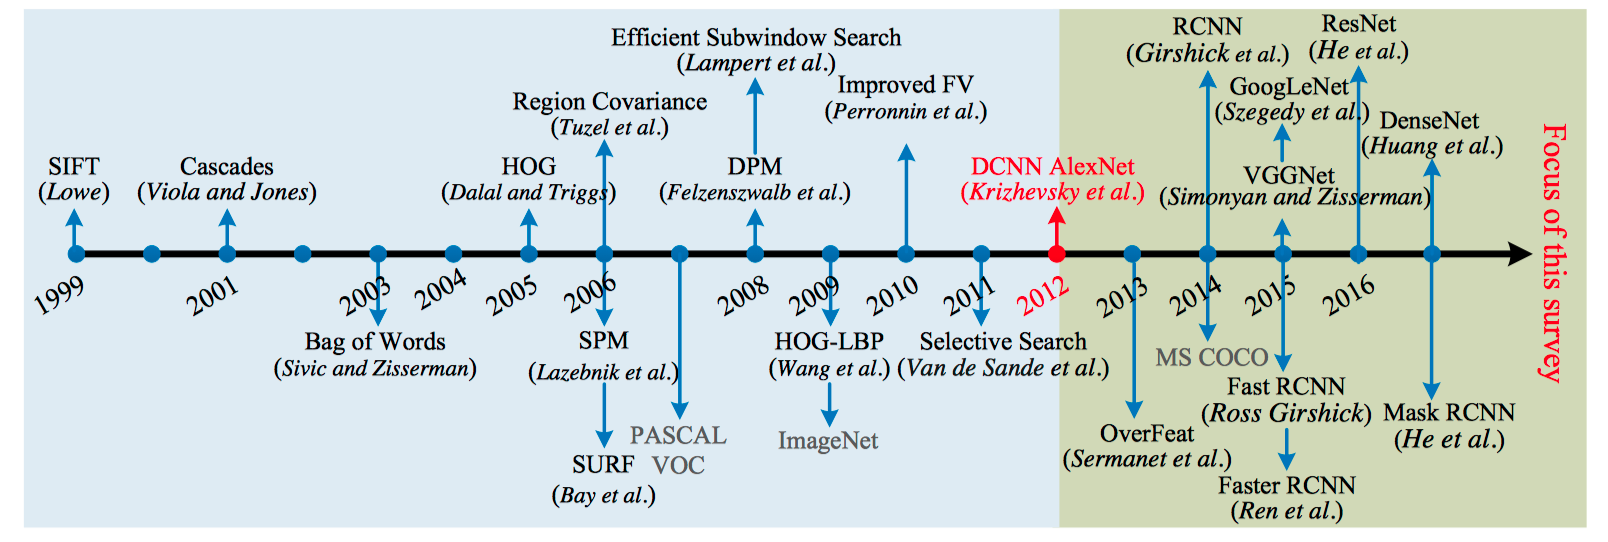
\includegraphics[width=\linewidth]{figures/timeline_od.png}
    \caption[Timeline of various methods proposed for object detection]
    {Timeline of various methods proposed for object detection
    ~\protect\cite{survey1-on-dl-od-2018}. The methods in blue area are the
    hand-crafted detector and the methods in green area are the deep
    learning-based approaches.}
    \label{fig:od-timeline}
\end{figure}

The world ``stage'' here means an independent process or a separate branch
within the deep network structure.
As their names imply, one stage approach finish the whole object detection
process in one shot indicating it will be faster than its two stages sibling
due to the fact that less computation being performed.
While the two stages approach has an independent process to propose the areas
where it may contain an object then perform detection on those places. The
existing of the area proposed stage takes more time but since it is elaborated
and can cover more potential area than the one-stage approach, it can gain
better results in the context of accuracy.
%As their names imply, one stage approach finish the whole object detection
%process in one shot indicating that it is faster but due to less computation
%the accuracy is less than the two stages approach which takes more time
%because
%it has an independent process to propose the areas where it may contain an
%object then perform detection on those places but can gain higher
%accuracy.
Determine to use which kind of detector depends on the realistic
requirement of the application. In this thesis, since we want real-time
processing ability, one stage detector will be a better choice and we mainly
focus on the YOLO v3 detector, the implementation detail will be explained in
the next chapter.

\subsection{Two Stages Detector}
\label{sec:related-worked-two-stages-detector}

Most of the two stages detectors follows the same methodology, first proposes a
bunch of candidate regions that may contain object(s) then using a CNN
(convolutional neural network) to extract feature descriptors of each region.
Finally, apply a classifier to the descriptors to indicate the object, if exists,
fall into which bin of the pre-defined categories.

\subsubsection{R-CNN}

R-CNN was the seminal work of employing CNN on object detection task, at that time
it was proposed, it boosted the accuracy from 35.1\% to 53.7\% on PASCAL
VOC dataset \cite{r-cnn-paper-2013}.
It designed a cascade pipeline contains four modules shown as
\autoref{fig:r-cnn}, named R-CNN stands for region with CNN features.
There are two important points this work brought to the table:
(1) it proposed a selective search method to find the possible candidates
replacing the old fashion sliding window way,
which improve the computation time significantly.
(2) it adopted CNN as feature extractor which can obtain more robustness
features rather than the hand-crafted one (like
only the color, texture, etc).

\begin{figure}
    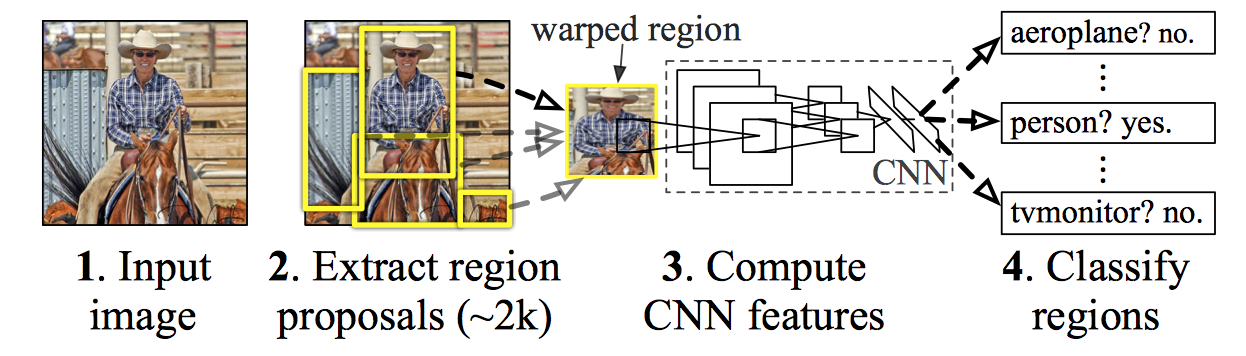
\includegraphics[width=\linewidth]{figures/r_cnn.png}
    \caption{R-CNN system overview ~\protect\cite{r-cnn-paper-2013}.}
    \label{fig:r-cnn}
\end{figure}

\subsubsection{SPP-net}

Even though R-CNN brought large margin of improvement into the object detection
research, it still has the potential to be
better observed by Kaiming He and his team who proposed
\cite{spp-net-paper-2014} one year after R-CNN being published,
which improved both runtime efficiency and accuracy compared with R-CNN. There
are two main issues from R-CNN which
they tried to address:

\begin{itemize}
    \item The generated candidate regions may have overlap which can lead to
    repeated computation of the same feature maps

    \item When ensuring the image to a fixed size, no matter cropping or warping,
    both have a large possibility that leads to information missing which can
    effect the training significantly
\end{itemize}

\cite{spp-net-paper-2014} solved the first problem by reverse the order of
selective search and convolution operation
and employed a special layer named ``spatial pyramid pooling" (SPP net) at the
end of the convolutional layer to eliminate
the second problem. By using SPP-net, the final feature maps will only be
computed once then pool features in arbitrary
regions to generate fixed-length descriptor for training, shown as
\autoref{fig:spp-net}.


\begin{figure}
    \begin{center}
    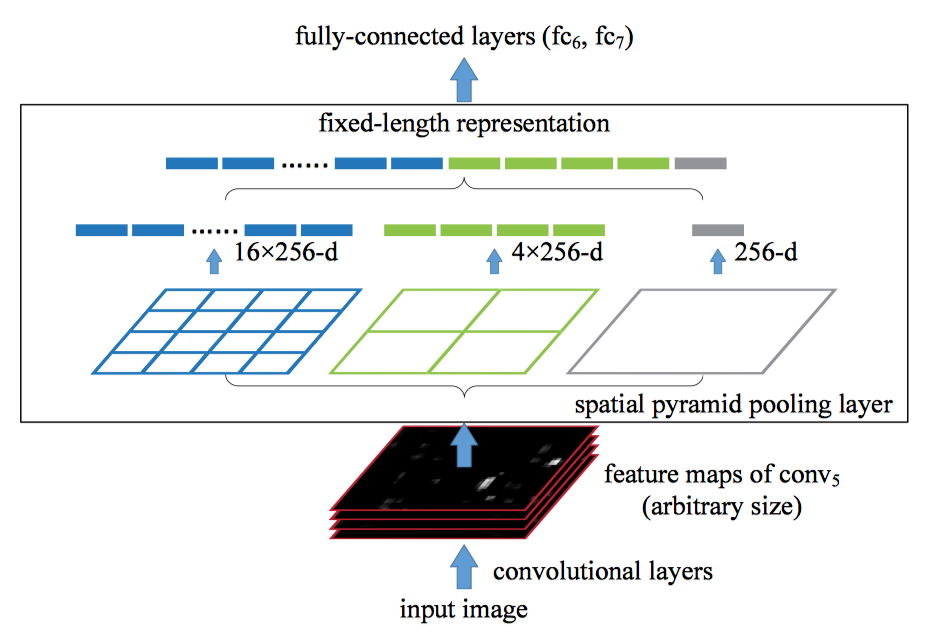
\includegraphics[scale=0.7]{figures/spp_net.png}
    \end{center}
    \caption{Illustration of how spatial pyramid layer works
    ~\protect\cite{spp-net-paper-2014}.}
    \label{fig:spp-net}
\end{figure}


\subsubsection{Fast R-CNN}

Fast R-CNN \cite{fast-r-cnn-paper-2015}, just like its name says, is
an advanced version of R-CNN, created by the same
author Ross Girshick independently. This update mainly focuses on speed up both
training and testing procedure, it targets
at not only R-CNN but also SPP-net for their common drawbacks:

\begin{itemize}
    \item The training pipeline is a multi-stages process
    \item Features are written to disk during training
    \item Object detection (testing) is slow
\end{itemize}

The solution for these issues is quite straight forward. Firstly, the author
changed the cascade pipeline to become a
parallel one, shown as \autoref{fig:fast-r-cnn}. Secondly, it modified the loss
to be a multi-task loss which reduces the
training complexity and makes all the layers updatable (the proposed fine-tuning
algorithm cannot update the convolutional
layer that precedes the spp layer). Third, the feature caching on the disk was
no longer needed.

\begin{figure}
    \begin{center}
    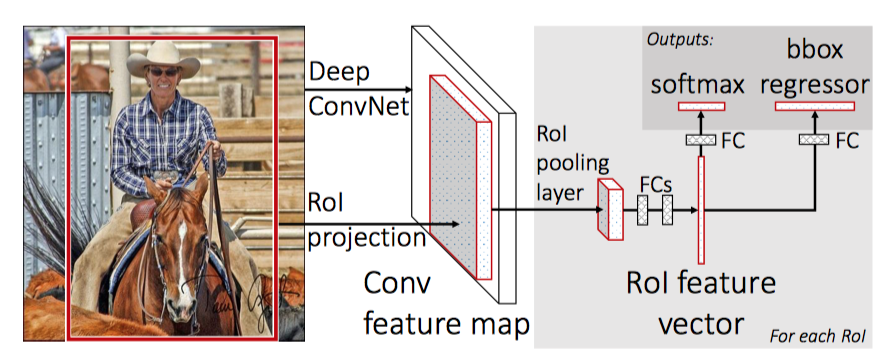
\includegraphics[scale=0.7]{figures/fast_r_cnn.png}
    \end{center}
    \caption{Parallel workflow of Fast R-CNN
    ~\protect\cite{fast-r-cnn-paper-2015}.}
    \label{fig:fast-r-cnn}
\end{figure}


\subsubsection{Faster R-CNN}

Faster R-CNN was a milestone of the usage of deep convolutional neural network
in the research of
object detection, it was created by the combination of teams which proposed
R-CNN and SPP-net. Before it came up,
the candidate regions were calculated via a method called selective search. But
in \cite{faster-r-cnn-paper-2015},
they introduced a region proposal network (RPN) which was embedded as a branch
into the model can learn how to
produce reliable candidate regions during the training time, the overall
structure of Faster R-CNN shown
as \autoref{fig:faster-r-cnn}. By using such an architecture, the model can
achieve predicting bounding box of the object
and computing the objectness score simultaneously (through one forward pass).
There are several advantages of
Faster R-CNN compared to its previous works:

\begin{itemize}
    \item Deep learned features are more reliable than the selective search one
    \item The whole network can be trained end-to-end
    \item The whole pipeline can be done on GPU (selective search need to be
    done on CPU before) which can speed up the training time
\end{itemize}

\begin{figure}
    \begin{center}
        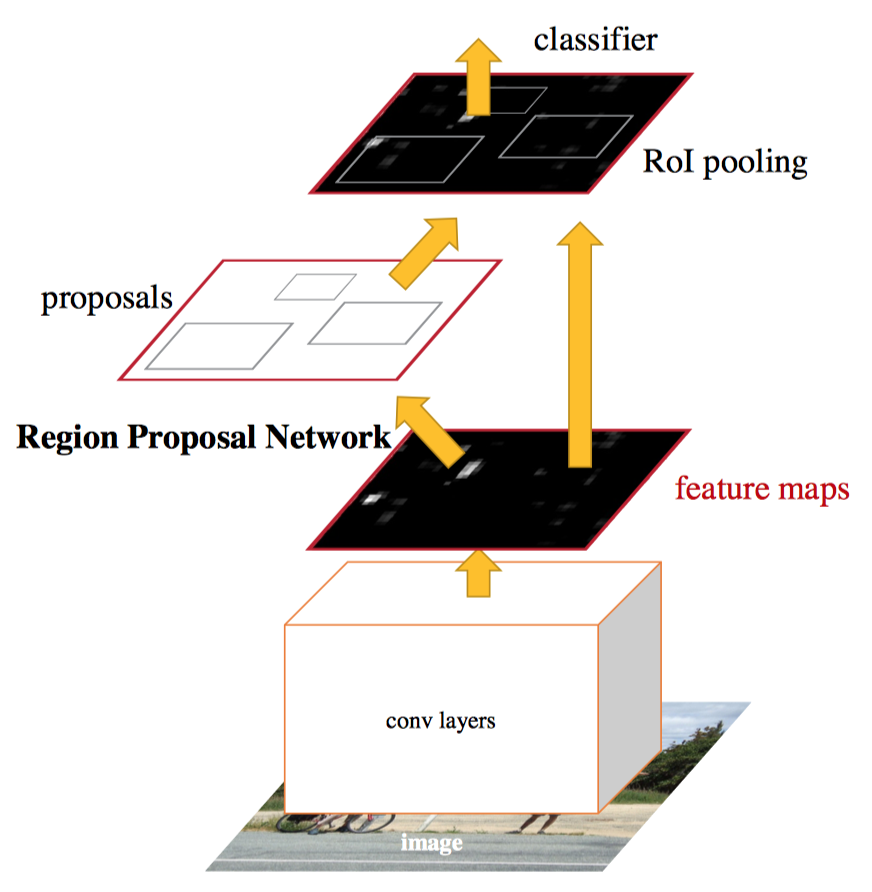
\includegraphics[scale=0.5]{figures/faster_r_cnn.png}
    \end{center}
    \caption{Structure of Faster R-CNN ~\protect\cite{faster-r-cnn-paper-2015}.}
    \label{fig:faster-r-cnn}
\end{figure}

There is one more thing needs to be pointed out, this work introduced the
concept of ``anchor'' which would be widely
used in the latter objection detection research including the one stage
detector we are going to review in the next subsection.
At each sliding-window position, the network would simultaneously predict $k$
region proposals which relative to
$k$ reference bounding boxes, these reference boxes are called anchor, one example
can be shown as \autoref{fig:anchor}.

\begin{figure}
    \begin{center}
    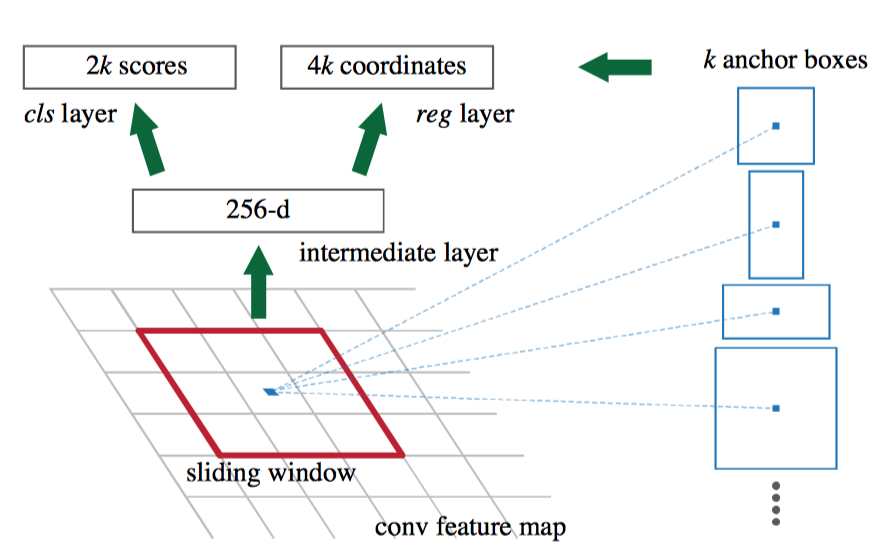
\includegraphics[scale=0.6]{figures/anchor.png}
    \end{center}
    \caption{Illustration of anchor mechanism
    ~\protect\cite{faster-r-cnn-paper-2015}.}
    \label{fig:anchor}
\end{figure}


\subsubsection{Mask R-CNN}

The most recent work of these object detection research family was called Mask
R-CNN \cite{mask-r-cnn-paper-2017} proposed
by Kaiming He again. It was not only an object detection network but also can be
used in the object segmentation domain. The idea
is that (1) it added another mask branch into the network to create a mask for
each detected object instance and (2) using a
more advanced backbone network for feature extraction (e.g. ResNet and FPN),
its architecture shown as \autoref{fig:mask-r-cnn}.
Again, the loss used to guide the training is the multi-task loss from Faster
R-CNN with the mask loss added expressing as:
$L = L_{cls} + L_{bbox} + L_{mask}$. Another creative idea, ROI alignment, is
notable to mention can improve
accuracy for bounding boxes regression.

\begin{figure}
    \begin{center}
    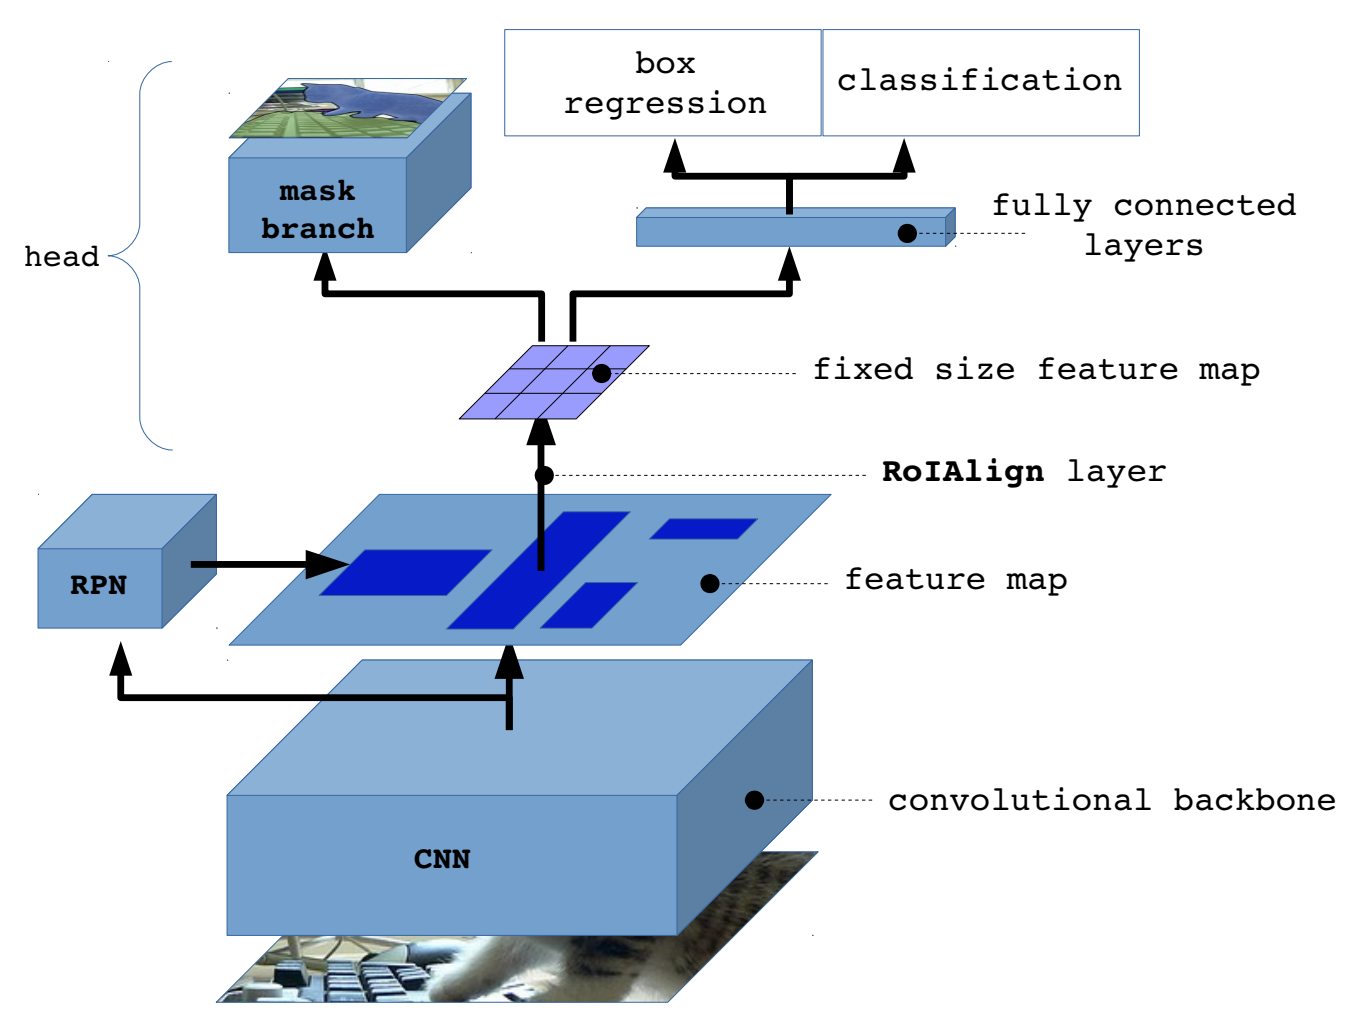
\includegraphics[scale=0.5]{figures/mask_r_cnn.png}
    \end{center}
    \caption{Architecture of Mask R-CNN ~\protect\cite{mask-r-cnn-slide}.}
    \label{fig:mask-r-cnn}
\end{figure}


\subsection{One Stage Detector}
\label{sec:related-worked-one-stage-detector}

One stage detector refers to those who directly predict class score and bounding
box offsets from the input with a single feed-forward CNN network. There is no
separate region proposed process exists at all, all the computations are done
within just a single network which can be optimized end-to-end directly on
detection performance.

\subsubsection{YOLO}
\label{sec:related-worked-yolo}

YOLO stands for you only look once, which indicates that it is a one-stage
object detector. Until now, there is a total of
three versions of the YOLO algorithm, YOLO v1, YOLO v2, YOLO v3 were published
in 2015, 2016, 2018 respectively. Compared
with the R-CNN series methods, YOLO doesn't have the stage of candidate region
calculation. It used a single network to
directly output the objectness score and the bounding boxes if objects exit.

\textbf{YOLO v1} \cite{yolov1-paper-2015}, this work was the fundamental
building block of the latter YOLO's algorithm
which just borrowed or added advanced techniques or tricks to improve the
performance. The workflow of the algorithm can
be summarized as the following steps and visualized as
\autoref{fig:yolo-v1-workflow}:

\begin{itemize}
    \item Take the input image (with size $448 \times 448$), cut it into $S
    \times S$ grids, each of them is responsible for detecting those objects
    whose center located within this grid

    \item Each grid will predict $B$ (an integer) bounding boxes and the
    confidence score of each box, for each predictive bounding box, the result
    should be a five-dimensional vector $(x, y, w, d, c)$

    \item For each grid (no matter how may bounding box is required), it should
    also output a probability for all required classes (if the dataset contains
    10 classes of object, it should output a probability for each class which
    means 10 probabilities in total)

    \item Sort all the result and use a threshold to filter out the detected
    bounding boxes whose probability lower than it
\end{itemize}

\begin{figure}
    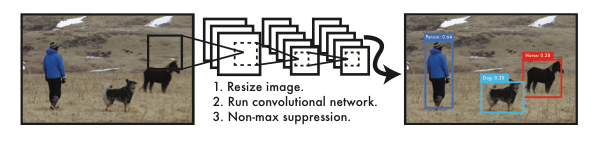
\includegraphics[width=\linewidth]{figures/yolo_v1_workflow.png}
    \caption{Workflow of YOLO v1 ~\protect\cite{yolov1-paper-2015}.}
    \label{fig:yolo-v1-workflow}
\end{figure}

An example process for an input image can be shown as
\autoref{fig:yolo-v1-example}, from that figure we can find that the
class score computation and bounding box prediction happened parallel. At
the end, another common technique, non-maximum
suppression \cite{non-maximum-suppression-paper} was applied to eliminate the
duplicated boxes point to the same object.
In the implementation point of view, the YOLO series was written in pure C from
sketch, the author provided his own framework
named Darknet \cite{darknet13} for his own deep neural network including
backbone network, optimizer, parameters update
methods, etc. The backbone network's architecture shown as
\autoref{fig:yolo-network}, it was a 24 convolutional layers
with 2 dense layers appended. The whole network was pre-trained on ImageNet
with resolution $224 \times 224$ then
double the size for detection.


\begin{figure}
    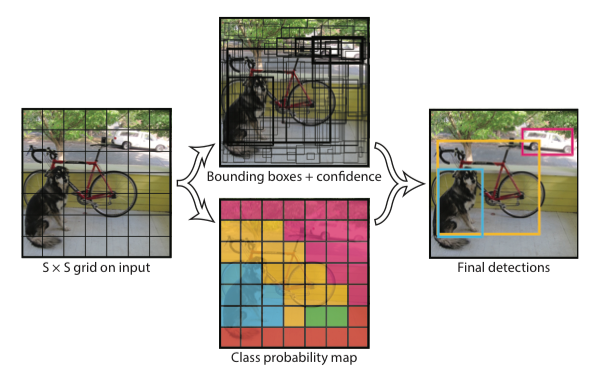
\includegraphics[width=\linewidth]{figures/yolo_v1_grid_example.png}
    \caption{An process example YOLO v1 ~\protect\cite{yolov1-paper-2015}.}
    \label{fig:yolo-v1-example}
\end{figure}

\begin{figure}
    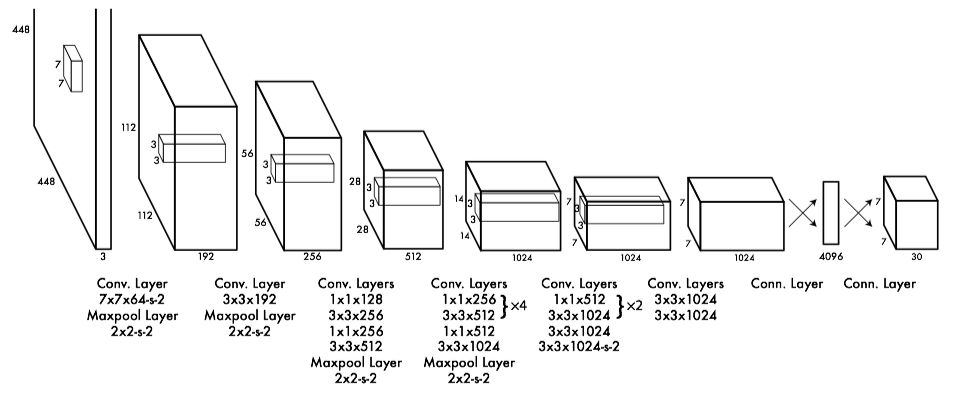
\includegraphics[width=\linewidth]{figures/yolo_v1_network_architecture.png}
    \caption{YOLO v1 network architecture ~\protect\cite{yolov1-paper-2015}.}
    \label{fig:yolo-network}
\end{figure}

\textbf{YOLO v2} \cite{yolov2-paper-2016}, this work is an update of it
previous version to improve the performance while
keeping its advantage which is fast (67 FPS vs. 5 FPS for Faster R-CNN), a
comparison can be found at \autoref{fig:yolo-v2-s-acc}.
There are a lot of works being done to make it works:

\begin{itemize}
    \item Added batch normalization layer to gain 2\% mAP improved.

    \item Pre-train on ImageNet directly using images with size $448 \times
    448$ (double from v1), increasing 4\% mAP.

    \item Introduced convolutional ``anchor'' boxes from Faster R-CNN which
    bring 7\% recall improvement.

    \item During training, every 10 epochs change the scale of images to obtain
    more powerful generalization ability.

    \item $13 \times 13$ resolution feature map is enough for ordinary objects
    but in order to overcome the disadvantage from v1 that perform poorly on
    small objects, a passthrough layer has been added that bring the feature
    from an earlier layer at $26 \times 26$ resolution.

    \item Proposed a new backbone network called Darknet-19, which has 19
    convolutional layers and 5 maxpooling layers.
\end{itemize}

\begin{figure}
    \begin{center}
    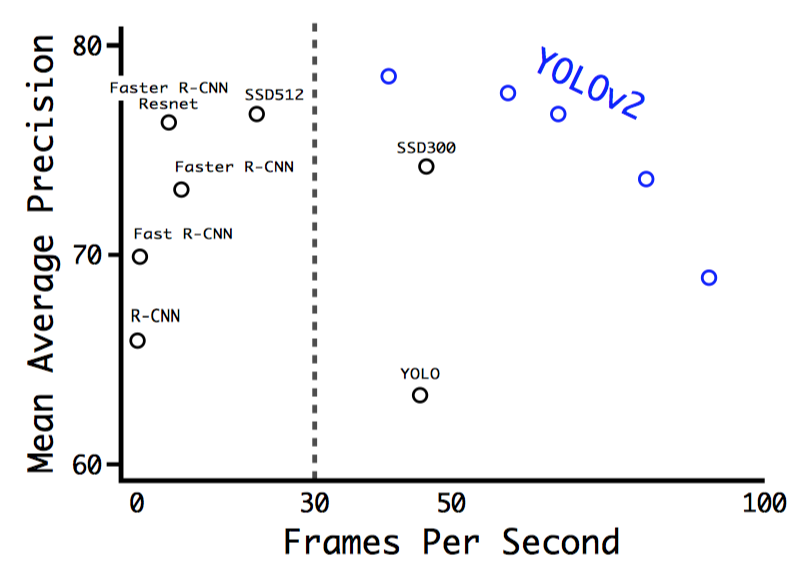
\includegraphics[scale=0.7]{figures/yolov2_speed_and_acc.png}
    \end{center}
    \caption{YOLO v2 accuracy and speed on VOC 2007 dataset
    ~\protect\cite{yolov2-paper-2016}.}
    \label{fig:yolo-v2-s-acc}
\end{figure}

\textbf{YOLO v3} proposed by \cite{yolov3-paper-2018}, according to the author,
it was not a research paper but a
technical report. It again pushed the speed and accuracy into a notable line,
\autoref{fig:yolo-v3-comp} shown
the comparison of the inference time of YOLO v3 with most of existing
comparable methods.

\begin{figure}
    \begin{center}
        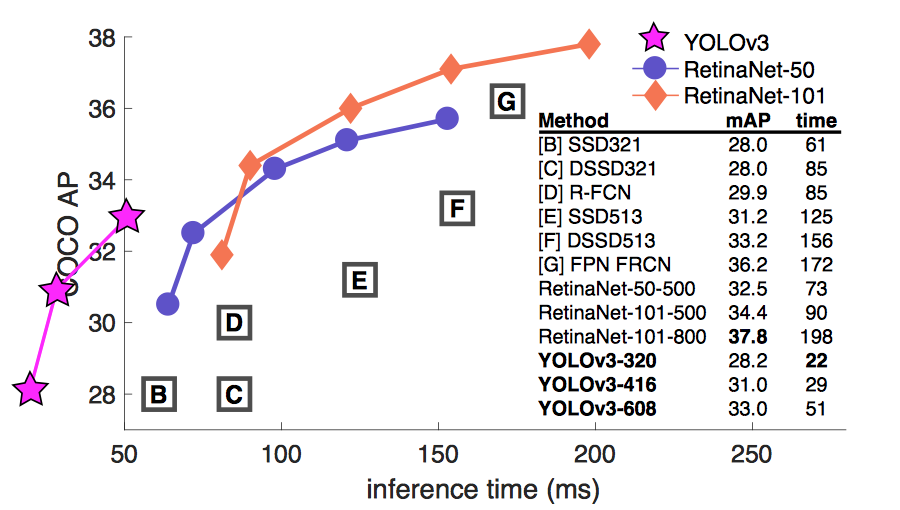
\includegraphics[scale=0.7]{figures/yolov3_comp.png}
    \end{center}
    \caption{Inference time of YOLO v3 compare with others
    ~\protect\cite{focal-loss-for-dense-od}.}
    \label{fig:yolo-v3-comp}
\end{figure}

According to their paper, there were some significant changes applied in this
version:

\begin{itemize}
    \item It designed a new backbone classification network that depends on the
    works of Residual Network from \cite{resnet-paper1-2015}
    \cite{resnet-paper2-2016} named Darknet-53 which can improve the top1
    accuracy about 3.1\% while maintaining the speed of 78 FPS.

    \item It discarded the softmax for classification instead using a simple
    logistic classifier, during the training, binary cross-entropy loss was
    employed which can solve the problem of overlapping labels (i.e. man and
    person) in a more complex dataset.

    \item It adopted a similar concept of feature pyramid networks (FPN) to
    enhance the scale-invariant ability of the model.
\end{itemize}

\subsubsection{SSD}

Five months after YOLO v1 being published, another famous one-stage approach,
named single shot detector (SSD) was
proposed by \cite{ssd-paper-2015}. It achieved much higher performance on mAP
metric than YOLO v1, precisely, 72.1\%
mAP on VOC2007 dataset at 58 FPS with $300 \times 300$ input size while YOLO v1
only have 63.4 \% at 45 PFS with
$448 \times 448$ input size, \autoref{fig:ssd_yolo_net} shows the architecture
difference between YOLO v1 and SSD.
To obtain these performances, the following three points contributed a lot:

\begin{itemize}
    \item Employed ``mechanism'' mapping object detection problem to finding a
    set of pre-defined bounding boxes.

    \item For each anchor, predict the class label and the offset of the
    boxes to locate the object better.

	\item For each input, combine feature map with different scales in order to
	      handle objects in various scales.
\end{itemize}

\begin{figure}
    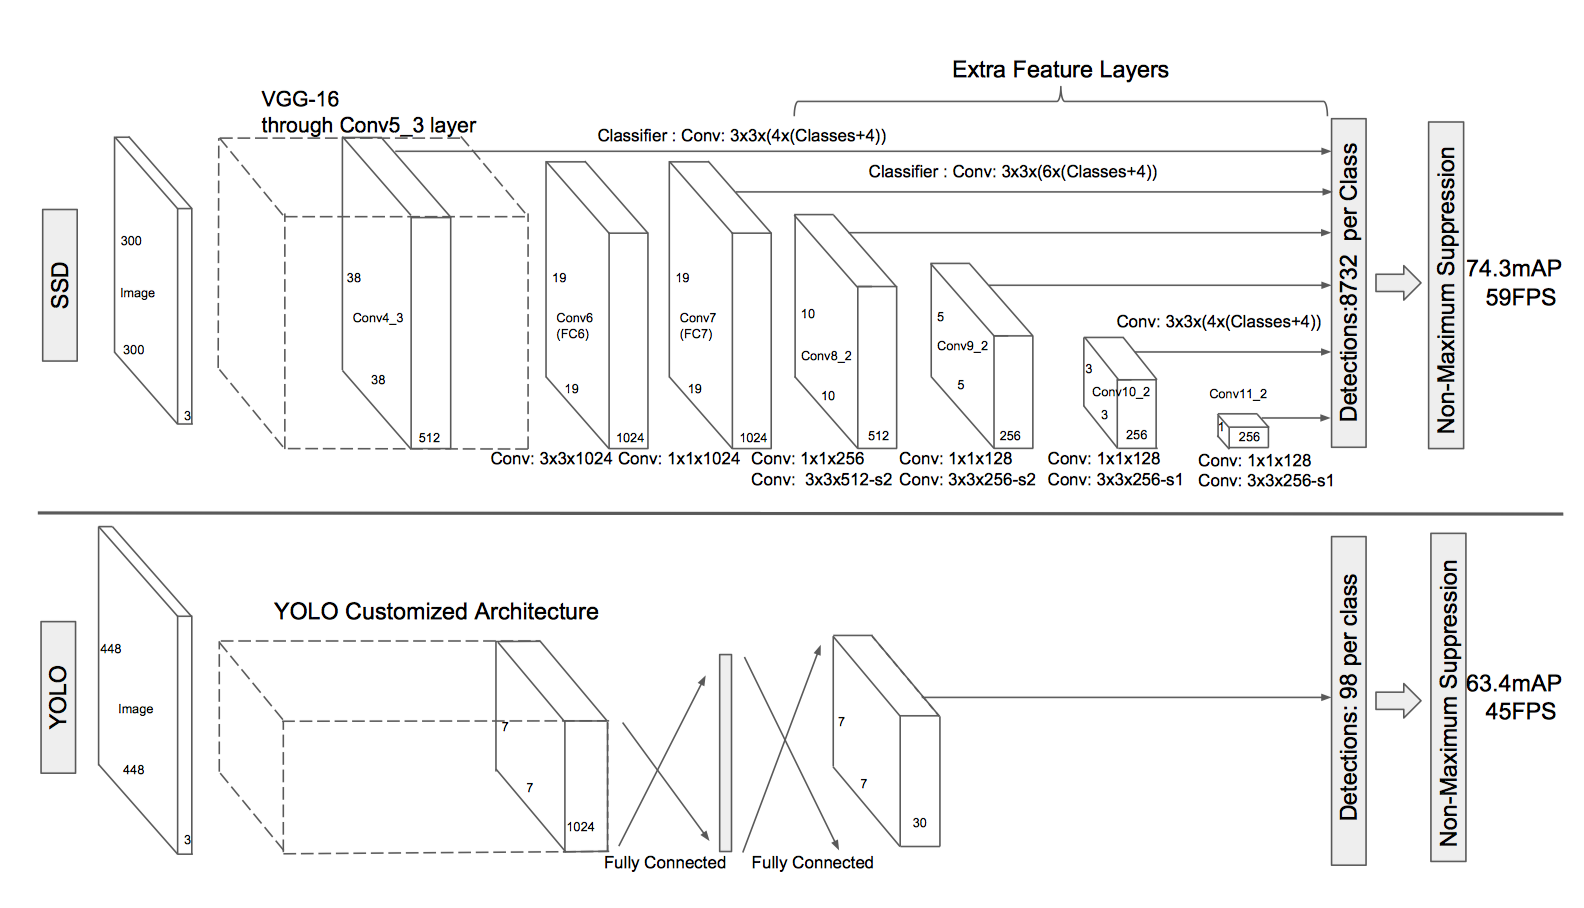
\includegraphics[width=\linewidth]{figures/ssd_yolo_net_arch.png}
    \caption{Network architecture comparison between SSD and YOLO v1
    ~\protect\cite{ssd-paper-2015}.}
    \label{fig:ssd_yolo_net}
\end{figure}

\section{Person Re-Identification}
\label{sec:related_work_re_id}

According to \cite{survey-reid-past-present-feature-2016}, the first definition
of person re-identification was given by Alvin Plantinga in 1961, from his
discussion of the relation between mental state and behavior. It was saying
that:

\begin{quotation}
``To re-identify a particular, then, is to identify it as (numerically) the
same particular as one encountered on a previous occasion.''
\end{quotation}


According to \cite{survey-on-dl-for-reid-2019}, let $\delta=\{\delta_1, ...,
\delta_M \}$ represents $M$ descriptors within a gallery set, given a probe
descriptor $U$, the identity of this probe person can be formulated as:

\begin{equation}
\label{general-reid-formula}
I = \arg_{\delta_i} \min (dis(\delta_i, U)),  \: \delta_i \in \delta
\end{equation}

where $I$ represent the identity of $U$ and $dis$ means a proper distance
function which will return the distance between $U$ and $\delta_i \in \delta$.
From \autoref{general-reid-formula}, we should notice that there are two key
points of the ReID task:

\begin{itemize}
    \item Feature descriptor
    \item Distance function
\end{itemize}

How to obtain suitable feature descriptors is always an interesting research
problem in the computer vision area. The traditional way to do it, of course, is
the hand-crafted descriptor which designed by the experts in this domain, for
example, BRIEF, SIFT, SURF, and ORB descriptors. All these are hand-crafted
descriptors and work well in their own purpose. But for various tasks, different
descriptors need to be created, obviously, it requires a lot of work and not
that convenient.

Since 2012, AlexNet \cite{imagenet-classifi-cnn} got a huge success in the
ImageNet classification competition, deep learning started boosted, using deep
neural network as feature extractor becomes popular and its performance defeats
most of the descriptors created manually. In the ReID community, more and more
researcher move their attention to the deep learning-based features (statistic
shown in \autoref{fig:papers-trend}) and a lot of creative methods were
developed based on (deep) neural network.

\begin{figure}
    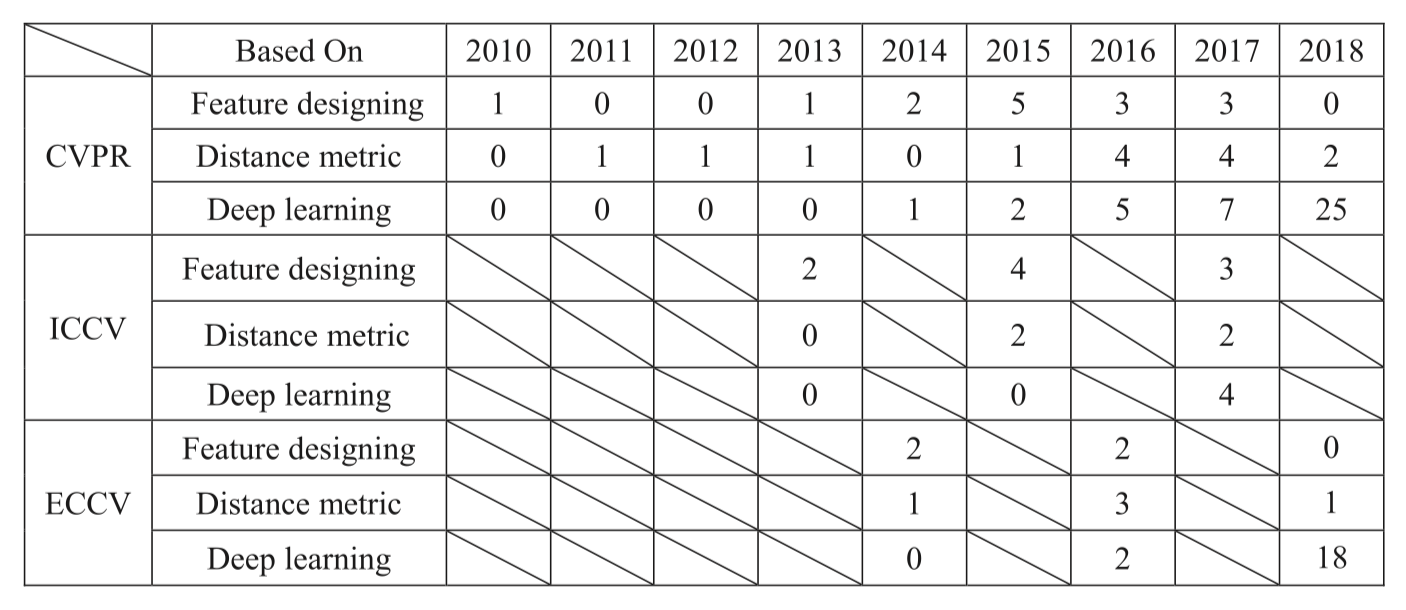
\includegraphics[width=\linewidth]{figures/papers_trend.png}
    \caption{The number of ReID papers depend on different approaches included
    by the three top conferences in recent years
    ~\protect\cite{survey-on-dl-for-reid-2019}.}
    \label{fig:papers-trend}
\end{figure}

In this section, we are going to review the existing deep learning-based approaches
for the ReID task, most of them can be separated into the following categories
\cite{survey-on-dl-for-reid-2019}:

\begin{itemize}
    \item Identification model
    \item Verification model
    \item Distance metric-based model
    \item Parts-based model
    \item Others
\end{itemize}

We will go deeper into each of these different models in the following
subsections, but mainly concentrate on the identification model and the
distance metric-based model, because our implementation which will be
introduced in the next chapter exactly is a combination of these two models.


\subsection{Identification Model}
\label{sec:related-work-re-id-idm}

Identification model regards the ReID task as the classification task, distinct
identities will be seen as different classes, the basic architecture of the model
is shown as \autoref{fig:id-model}. The input to the
network will be the output from some kinds of person detector, then the deep
neural network (e.g. CNN) severs as a feature extractor and by making use of these
extracted features the input image will be tagged
with an identity.

Due to the lacking of data, the main issue of the classification model in deep
learning is always overfitting which means that the model performs pretty good on the
training set but poor on the validation set. Especially on the ReID task, we want more
training samples for each individual but most of the dataset only have few sample
per instance (e.g. VIPeR only contains two images per identity). A lot of works had
been done to solve this problem, they can be roughly categories into
(1) add other constraints to revise overfitting,
(2) apply data argumentation techniques or create large datasets.

\begin{figure}
    \begin{center}
    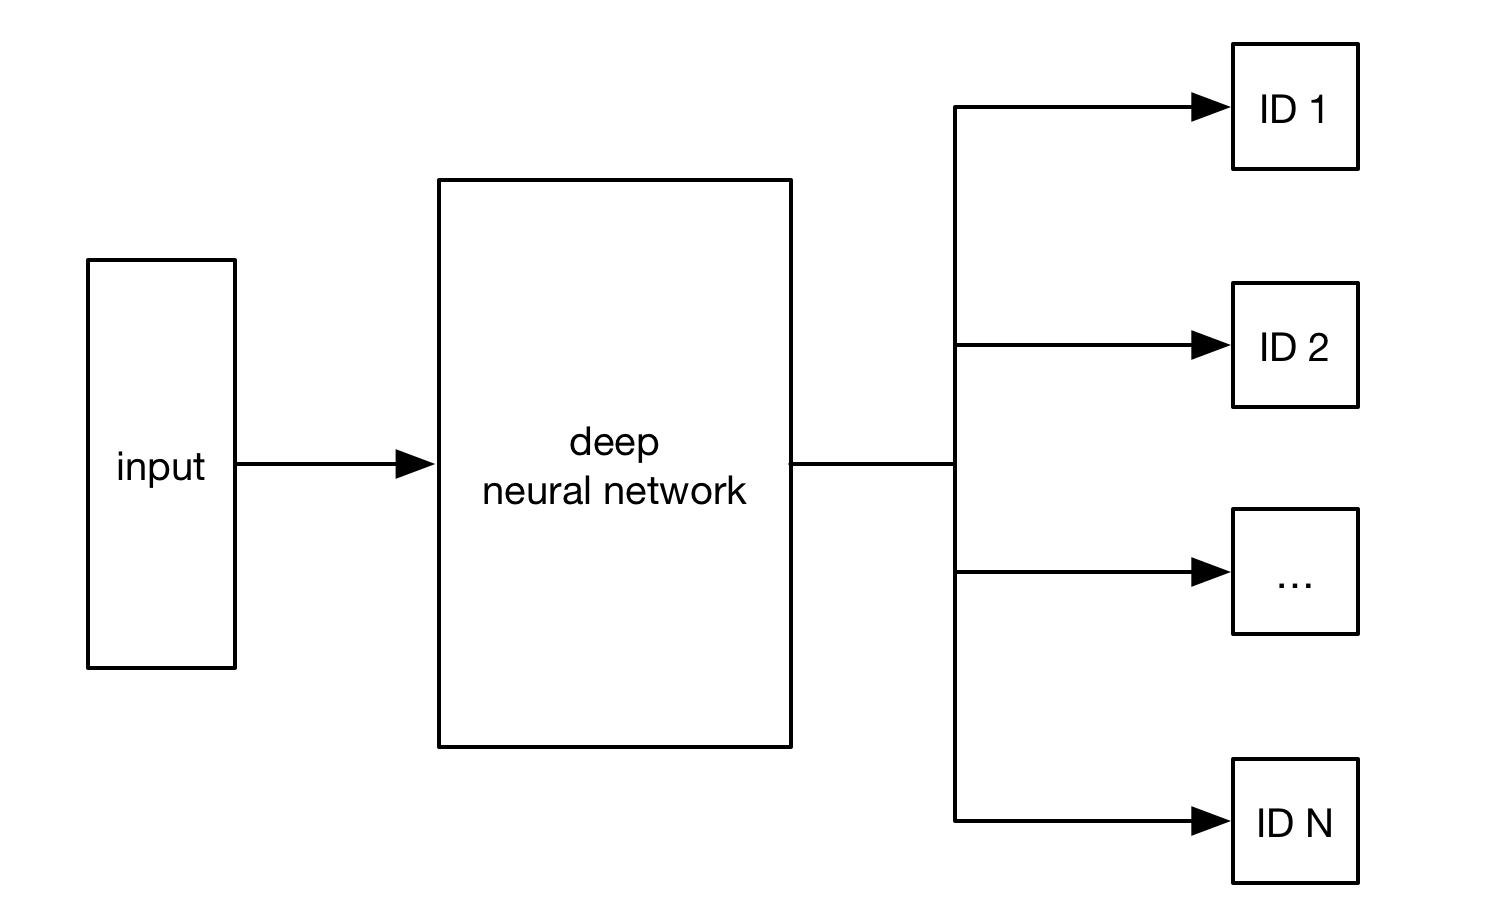
\includegraphics[scale=0.8]{figures/id_model.png}
    \end{center}
    \caption{Architecture of identification model.}
    \label{fig:id-model}
\end{figure}

In \cite{feature-fusion-net-2016}, the authors proposed a fusion feature
network (FFN), which can take the CNN features and the hand-crafted feature into
consideration at the same time, its architecture is shown as
\autoref{fig:ffn}. FFN takes the identity image as input then branch into two
paths. For the CNN feature, five layers convolutional network and two fully connected layers
were employed. For hand-crafted feature extraction, the original image was divided into horizontal
stripes then color spaces and texture filters were applied in order
to extract histograms which finally were concatenated to form a feature vector. At the end,
theses two kinds of feature would be linked together through another dense layer. The whole
network was trained under the softmax loss and during back-propagation parameters update would
also be constrained by the hand-crafted feature.

\begin{figure}
    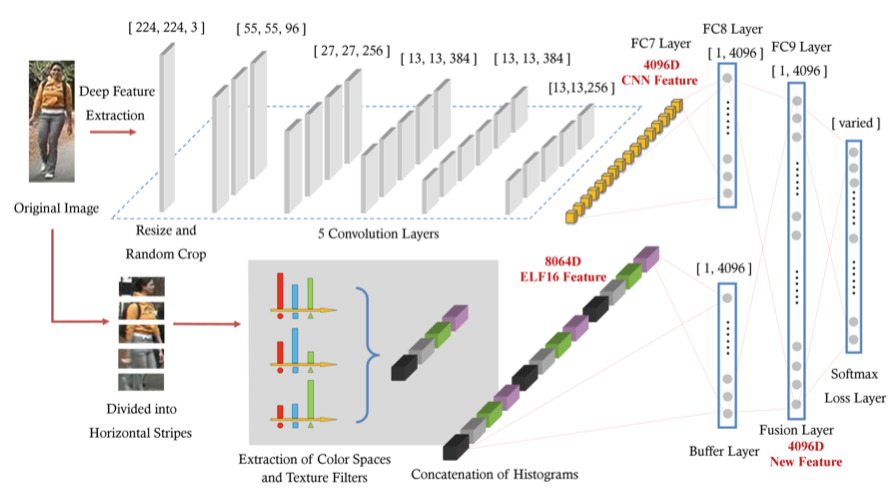
\includegraphics[width=\linewidth]{figures/ffn.png}
    \caption{Architecture of fusion feature network ~\protect\cite{feature-fusion-net-2016}.}
    \label{fig:ffn}
\end{figure}

The idea behind the classification model is that we are trying to use several hyperplanes
to separate different identities in the feature spaces. But since it is a high dimensional space,
in some cases, the intra-class variance may larger than inter-class variance which is not a good
property for a classification model. In order to enhance the learned discriminative feature,
\cite{hybrid-net-lda-2016} proposed a hybrid network architecture that combined with the Fisher
vectors which include color histograms and SIFT and a deep neural network.
%In our implementation, we also target to solve this problem,
%\cite{center-loss-2016}
%which originally proposed for face recognition called ``center loss"
%was employed. It maintains a center point of each identity
%and pushes each image embedding to its corresponding center so the
%variation between the same identity embedding is smaller.

It is worth to mention that when deep learning in ReID area becomes more and more popular,
there are several large datasets like
\cite{dataset-cuhk03-2014}, \cite{dataset-market1501-2015}, \cite{dataset-dukemtmc-2016} and
\cite{dataset-cuhk03-np-2017} have been released as well as their proposed evaluation protocols.
Since deep learning really depends on data, these datasets help the ReID research
community a lot. With the large dataset, we are able to train the network directly based on the
plain classification model. \cite{generic-deep-feature-for-reid-2016} trained the plain classification
network on multiple datasets with domain guided dropout strategy aiming at obtaining a cross-domain
model. Dropout is an implemented-friendly but useful technique  to prevent overfitting proposed
by \cite{dropout-paper-2014}.

Jointly learning is another hot topic in the deep learning community, it means the model is trained under
the guidance of two or even more loss (objective) functions. In specific ReID research,
\cite{comb-id-and-center-loss-2017} proposed a jointly learning method which adopt
identification loss and center loss \cite{center-loss-2016}, architecture shown as
\autoref{fig:comb-center-id-loss}. It claims that it is more efficient than the
pairwise or triplet model and the performance is also better by using their feature reweighting
layer (FRW). The core idea is that during the training the model tries to enlarge the inter-class variation
and reduce the intra-class variation supervised by the center loss while
the identification loss makes full use of the image label compared with the verification model which
just used the weak label information.

\begin{figure}
    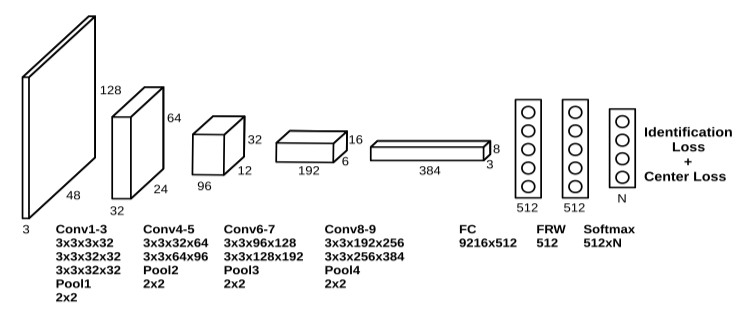
\includegraphics[width=\linewidth]{figures/comb-center-id-loss.png}
    \caption{Architecture of fusion feature network ~\protect\cite{comb-id-and-center-loss-2017}.}
    \label{fig:comb-center-id-loss}
\end{figure}

\subsection{Verification Model}

Verification Model can be seen as a classification problem as well but it is the binary version. It takes a
pair of images as input and output a similarity value indicating whether the paired images is the same
person or not. Its architecture shown as \autoref{fig:vft_model} and can be simply formulated as:

$$
f(x_1, x_2) =
\begin{cases}
1&  y_1 = y_2 \\
0&    y_1 \neq y_2
\end{cases}
$$

\begin{figure}
    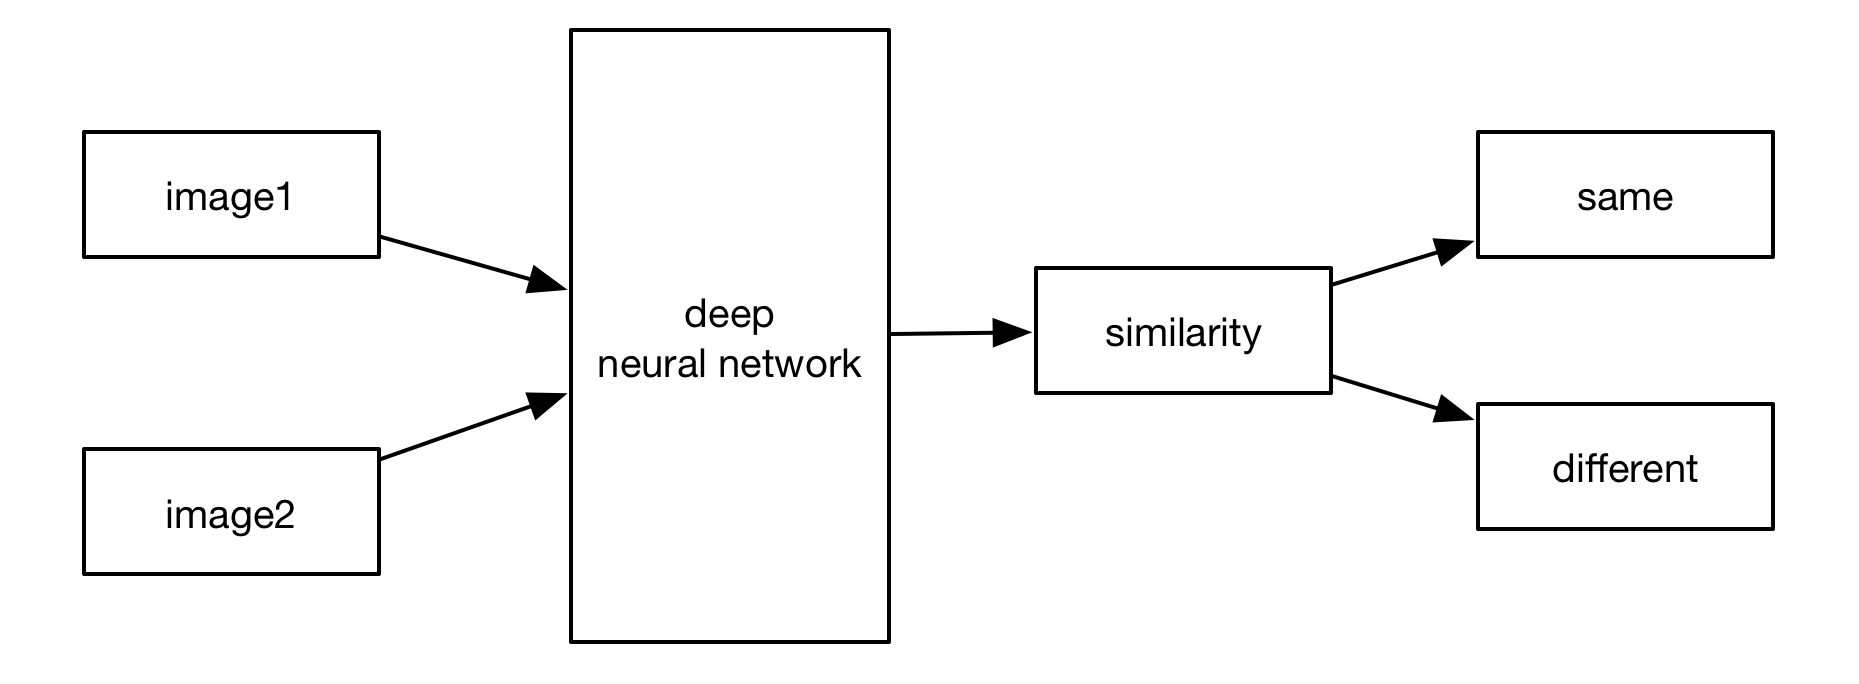
\includegraphics[width=\linewidth]{figures/verification_model.png}
    \caption{Architecture of verification model.}
    \label{fig:vft_model}
\end{figure}

\cite{first-pairwise-net-for-reid-2014} proposed the first verification model to address ReID task named filter pairing
neural network (FPNN). Max-out pooling layers and patch-matching were employed to jointly handle geometric
transforms and photometric, misalignment, background clutter and occlusions which are common issues in ReID domain.
At the time that where datasets are still extremely limited, ``Siamese" deep network for metric learning which was firstly
proposed by \cite{first-siamese-net-for-reid-2014} to target this problem. Like the common verification model, it takes an
image pair as input. Then pass them through three shared parameters but independent convolutional networks to perform operations
on three non-overlapping parts of the images. The extracted feature descriptor will be flattened by a dense layer then used to
compute the cosine distance which will be converted into a similarity value. If the value is greater than a hyper-parameter
threshold then the input pair will be considered as the same identity, otherwise different. Based on the previous two works,
\cite{an-improved-dl-archit-2015} comes up with an improved architecture shown as \autoref{fig:cvpr15_model} that include a layer to
calculate cross-input neighborhood differences which based on mid-level features to capture local relationships of the input
paired images.

\begin{figure}
    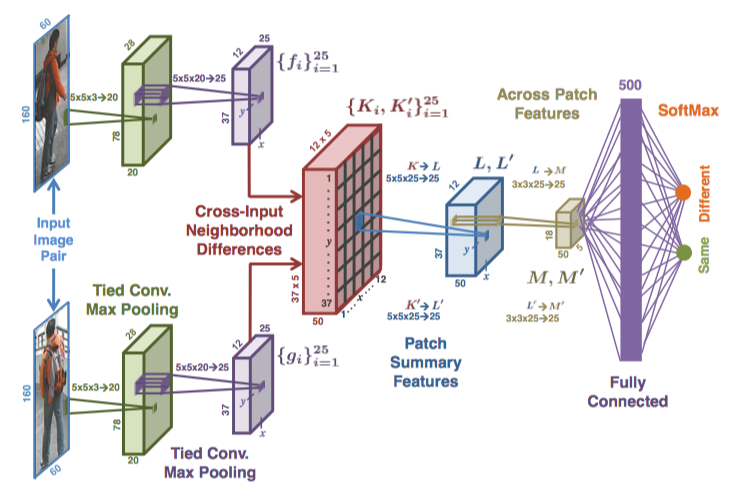
\includegraphics[width=\linewidth]{figures/cvpr15_model.png}
    \caption{Architecture proposed by ~\protect \cite{an-improved-dl-archit-2015}.}
    \label{fig:cvpr15_model}
\end{figure}

But these verification models introduced above all have a common problem which is that the neural network employed by them are relatively
shallow. By this limitation, it does not benefit from digging the features which are discriminative enough to distinct different identities.
Besides, since we have to construct the image pair for training, it will be some overhead added compared to the identification model. One more
thing is that the verification models only use the weak dataset label, which means that for a specific identity instance pair, it doesn't
care about their actual identity but they are the same or not. Unlike the identification model, it will tell directly which identity it is for each
given input.

Because of these limitations, only using the verification model may not achieve high accuracy in ReID task. Still, it is worth to mention
that the combination of identification and verification model can reach a promising result,
\cite{id-verif-combined-learned-cnn-embedding-for-reid-2016} proposed such a model and comprehensively compare the advantages and disadvantages
of these two models. They replaced contrastive loss by cross-entropy loss which is different from its sibling network on face recognition, then
applied dropout regularization to prevent overfitting.

\subsection{Distance Metric-based Model}
\label{sec:related-work-re-id-dism}
The distance metric-based model aims at making the distance between the same identity as small as possible while between
distinct identity as large as possible. One of the most popular used approaches is the triplet architecture.
A triplet unit of images can be defined as:
$I_i=\{I_i^1, I_i^2, I_i^3\}$,
where $I_i^1$ called anchor, $(I_i^1, I_i^2)$ is positive pair and $(I_i^1, I_i^3)$ is negative pair.
For each triplet unit, the model will try to satisfy the following:

\begin{equation}
    \label{eq:triplet-model-goal}
    \norm{F(I_i^1) - F(I_i^2)} ^2 < \norm{F(I_i^1) - F(I_i^3)} ^2
\end{equation}

where $\norm{}^2$ means the L2 norm and $F(I)$ denotes the features learned by the model. Based on \autoref{eq:triplet-model-goal}
we can define the loss as following:

\begin{equation}
    \label{eq:common-triplet-loss}
    L(I) = \sum_{i=1}^{n} \max\{ \norm{F(I_i^1) - F(I_i^2)} ^2 - \norm{F(I_i^1) - F(I_i^3)} ^2, C \}
\end{equation}

where $C$ is a non-negative constant, guided by \autoref{eq:common-triplet-loss}, the network will be forced to maximize the distance between
the anchor-positive and anchor-negative pair under L2 norm, the described procedure can be illustrated by \autoref{fig:triplet_objective}.

\begin{figure}
    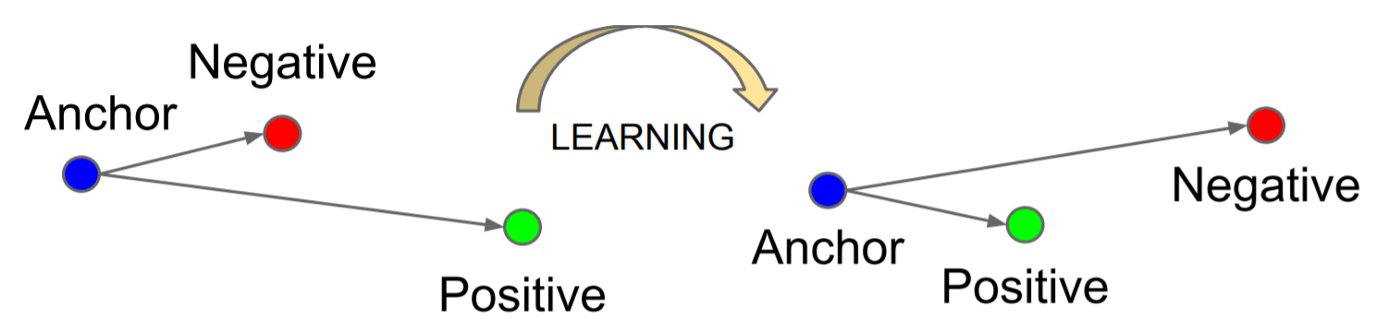
\includegraphics[width=\linewidth]{figures/triplet_objective.png}
    \caption{Objective of triplet loss ~\protect \cite{facenet-triplet-model}.}
    \label{fig:triplet_objective}
\end{figure}

In \cite{in-defense-of-triplet-loss-for-reid-2017}, comprehensive research had been conducted to the triplet model, covering the
strategy of sampling, different representations of the loss functions, comparison between pre-trained and plain model, etc. Some of their
methods are worth to mention in this paper:\\
(1) It proposed a novel way to sample the triplet unit, it says that randomly sample $p$ identities within the whole training set and for
each selected identity randomly pick $k$ instances per mini-batch.\\
(2) It came up with several representations of loss functions, the most popular two of them are batch-hard loss $L_{BH}$ and batch-all loss $L_{BA}$.
As their name stated, batch-hard loss means to find the hardest samples in the triplet and use them contribute to the loss while batch-all loss means all
the triplet units, no matter what they are, all contributing to the loss. They can be formulated as \autoref{eq:batch-hard}.

\begin{equation}
\label{eq:batch-hard}
     L_{BH} = \sum_{i=1}^{P} \sum_{a=1}^{K}
            [
                m + \max_{p=1...K} D(f_{\theta}(x_{a}^i), f_{\theta}(x_{p}^i))
                - \min_{\substack{j=1...P\\ n=1...K\\ j\neq i}}
                D(f_{\theta}(x_{a}^i), f_{\theta}(x_{n}^j))
            ]_+
\end{equation}

where $D$ is a distance function, $f_\theta$ is the feature descriptor, $m$ is a margin constant, $[\:]_+$ means the result within bracket will
be a non-negative number.

\begin{equation}
\label{eq:batch-all}
    L_{BA} = \sum_{i=1}^{P} \sum_{a=1}^{K}  \:
             \sum_{\substack{p=1\\ p\neq q}}^{K} \:
             \sum_{\substack{j=1\\ j \neq i}}^{P} \:
             \sum_{n=1}^{K} \:\:
             [m + d_{j, a, n}^{i, a, p}]_+
\end{equation}

$$d_{j, a, n}^{i, a, p} =  D(f_{\theta}(x_{a}^i), f_{\theta}(x_{p}^i)) - D(f_{\theta}(x_{a}^i), f_{\theta}(x_{n}^j))$$

Effectively, by using $L_{BH}$ we can have $PK$ terms contribute to the loss while using $L_{BA}$ we have $PK(PK - K)(K - 1)$ terms
contribute to the loss. It really depends on the realistic scenario to determine which loss we should choose. At this point, it is
significant to note that these two variations of the loss still respect to the standard triplet loss function \autoref{eq:common-triplet-loss}.

(3) During the training, they found that using the non-squared Euclidean distance is more stable than using the squared one which will make the
optimization more prone to collapsing and reduce the interoperability of the margin constant (can't be absolute distance any more).

\subsection{Parts-based Model}

At the very beginning, \cite{hand-crafted-part-based} proposed a hand-crafted part-based model for matching two images based
on the appearance. It partitions pedestrians into horizontal stripes to extract color and texture features. After that several
works \cite{part-based-triangle}, \cite{part-based-pictorial-structure} try some more sophisticated strategies to divide the
person into parts. But still based on hand-designed approaches. When deep learning comes to the picture, with the help of the
research from human pose estimation and landmark detection, the ReID part-based model achieves several impressed results
\cite{deep-part-based-glad}, \cite{pose-driven-dcnn-for-reid}, \cite{pose-invariant-embedding-for-reid}.

Attention mechanism is another milestone in the part-based model, the current statue of the art in ReID task is produced by it.
\cite{end-to-end-attention-network-for-reid} first adopted attention network to address ReID task, they proposed a LSTM-based
model using a recurrent approach that can output part attention feature dynamically for localizing discriminative regions of
the pedestrian image. One year after, \cite{hpnet-attentive-deep-feature-for-reid} comes up with a multi-directional
attention mechanism for capturing multiple attention information, the proposed network was named HP-Net.
For the part-based model, there is always a common issue which is the alignment problem. Once you divide the image into parts,
how to align these chunks and calculate the similarity properly will be problematic. To address the misalignment issue,
\cite{part-aligned-for-reid} introduces a CNN-based attention model that makes use of the distance between a paired image to
learn the part-feature for matching. In ECCV2018, \cite{pcb-and-rpp-for-reid} proposed a parted-based convolutional
baseline model (PCB) which employs a simple uniform partition strategy and assembles part-informed feature into a descriptor
and a refined part pooling (RPP) method which reinforce the within-part consistency introducing a large margin of improvement
without require any part labeling information, the architecture shown as \autoref{fig:rpp}.

\begin{figure}
    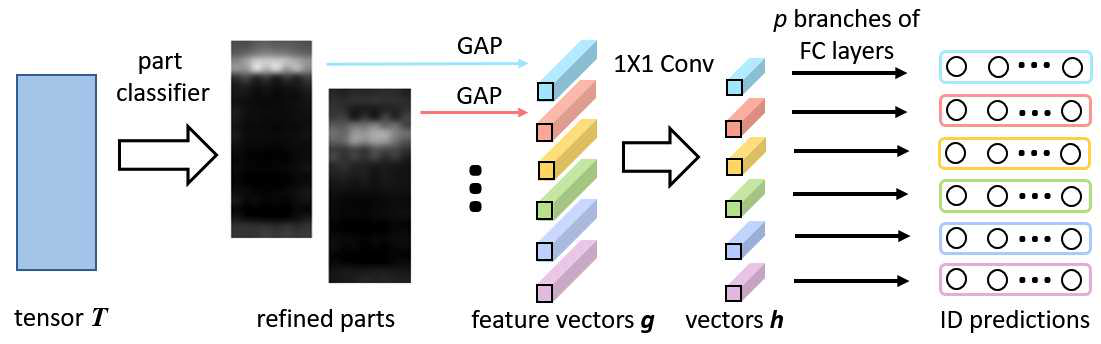
\includegraphics[width=\linewidth]{figures/rpp.png}
    \caption{PCB in combination of refined part pooling ~\protect \cite{pcb-and-rpp-for-reid}.}
    \label{fig:rpp}
\end{figure}

However, the part-based model still has its own limitations:

\begin{itemize}
    \item adding part-based branches reduces the efficiency of the model.
    \item most attention-based model only considers region-level attention and discard the pixel-level saliency.
    \item most of the model doesn't consider the spatial context information between different part-based features.
\end{itemize}

\subsection{Others}
\label{sec:related_work_other}

Besides the four major models described above, there are still some other deep learning-based researches on ReID community.
Even with the datasets like CUHK03, Market1501, and DukeMTMC-reID, the average numbers of image per person is still quite
limited. The first work try to enlarge the dataset with the generative adversarial network (GAN) was introduced by
\cite{first-gan-for-reid}, they employed GAN to generate unlabeled samples and adopt a CNN to extract feature for
representation learning. Then label smoothing regularization is used for outliers method.

\cite{camera-style-adaptation-for-reid} proposed a camera style adaption model to adjust the CNN training. More precisely,
CycleGAN is used to transfer the style of images captured by one camera to another. Given an image from camera No.1, the model
can produce the image which looks like captured by camera No.2.

Unlike most of the works which are based on RGB image, it is noteworthy to mention a work which employs RGB-D data as input.
\cite{rgbd-for-reid} introduced a novel method for ReID using RGB-D data, the proposed pipeline shown as \autoref{fig:rgbd-pipeline}.
It takes a RGB-D image as input, then performs a segmentation to obtain different parts of the human body, using this information
to do 3D reconstruction and pose transformation resulting with a standard human 3D model. Then using the attributes computed from
the 3D model to perform re-identification.

\begin{figure}
    \begin{center}
        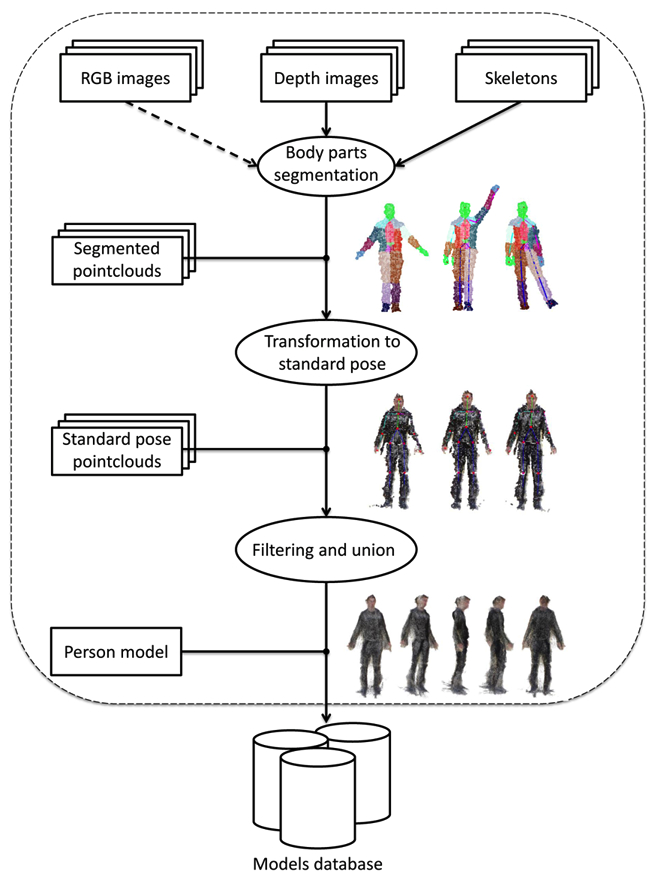
\includegraphics[scale=0.4]{figures/rgbd_for_reid.png}
        \caption{The working pipeline for ReID with RGBD data ~\protect \cite{rgbd-for-reid}.}
        \label{fig:rgbd-pipeline}
    \end{center}
\end{figure}

%\section{OpenISS Framework}
\section{Available Software}
\label{sec:related_work_framework}

The most impressive depth camera to people nowadays may still be the Microsoft Kinect, even it has been dropped
by its own company now. It was the first consumptive depth camera in the market released in Nov 2010. Kinect was
designed for Microsoft Xbox 360, a video game console. In order to let the game designer to fully make use of it,
a corresponding closed source library (known as Microsoft Kinect Develop Toolkit) was also released to enable
the programmability of the device.

\subsection{Freenect and Freenect2}
\label{sec:related_work_openiss_freenect}

Since the Microsoft Kinect Develop Toolkit is closed source and can only be used on the Windows machine. A group of
people from the community makes an open-source driver for Kinect named Freenect to enable it works on Linux, MacOS
and Windows. By using this Freenect driver, people can obtain the raw depth data from the device directly, a lot of
researches based on depth data boost increasingly since then. When Microsoft released Kinect v2 (the second version
of Kinect), the community also comes up with the driver Freenect2 with the same functionality.

\subsection{OpenNI2}

OpenNI or Open Natural Interaction library was originally found by PrimeSense which is a depth-sensing solution
provider company. Kinect was using their technology to obtain the depth data from the sensors. After the
acquisition of PrimeSense by Apple, they shut down the official website but the community (like Occipital and
other former partners) is still keeping a forked version of OpenNI2 active as
an open-source library for their product.

By using the OpenNI2 framework, we can access the following data using the
same unique APIs, if the hardware driver respect to the OpenNI2 standard.
Fortunately, both Freenect and Freenect2 have
the option to build an OpenNI2-supported version of them:

\begin{itemize}
    \item Voice and voice command recognition
    \item Hand gestures
    \item Body motion tracking
\end{itemize}

\subsection{OpenCV}
OpenCV is a library of programming functions mainly for computer vision. It
was originally created by Intel (for image processing) in 2000 and now lead by
Itseez. The library is cross-platform and open source under the BSD license,
widely supports most of the existing operating systems. The library was originally
written in C, but since 2009 it primarily changed to C++. Nowadays, it
also adds CUDA-based and OpenCL-based GPU calculation, machine learning and
deep learning (TensorFlow, Torch/PyTorch and Caffe) support.

\subsection{NiTE2}
\label{sec:related_work_openiss_nite2}

NiTE2 is a piece of middleware of OpenNI2 library, it has to work with OpenNI2
underneath and provide more powerful functionality than OpenNI2 does. It is
also the design philosophy of OpenNI2 which only supposed to provide the
infrastructure and leave all the other functionalities to the middleware.
Unfortunately, NiTE2 is a closed source library provided by PrimeSense, it was
written in C++ and only comes with the header file and the binary library. By
using NiTE2, we can get the following data:

\begin{itemize}
    \item Skeleton data of the tracked full human body
    \item Gesture data of the tracked hand
\end{itemize}

\subsection{RealSense SDK}

RealSense SDK is a cross-platform library from Intel for their own depth
cameras. The SDK allows the developer to access depth and color streaming and
provide the basic camera parameters for calibration. Since the SDK is provided
by the manufacturer directly which means they know everything about the
hardware, it is more powerful than Freenect and Freenect2 as to Kinect. The SDK
is written by C++ and hosted on GitHub, when this thesis is writing, the
community is still quite active and they still try to add more functionalities
to the SDK (like support OpenNI standard, working with OpenCV library, provide
more wrapper for other programming languages rather than C++).

\subsection{CPython}
\label{sec:related_work_cpython}

Our proposed OpenISS framework is designed to be written in C++ since most of
its dependencies list above are in C++. But nowadays, most of the deep learning
programs are written in Python, and for experiment and prototype purposes,
Python has a more efficient development environment. In order to invoke the
deep learning model from OpenISS framework, we need something to connect C++
and Python. CPython is our desired bridge, it is the reference implementation
of the Python programming language written in C and Python. It has a foreign
function interface with support to several other programming languages and C is
one of them. By making use of CPython we can exchange a class, a function, a
variable or other data structure with the languages on two sides of the bridge.

\subsection{TensorFlow}
\label{sec:related_work_openiss_tf}

Since deep learning get boosted recently, there are various of deep learning
frameworks being developed, \autoref{fig:dl-frameworks} shows the popularity of
most of the existing platforms. TensorFlow \cite{tensorflow2015-whitepaper} is
an open-source library written in C++ which designed by Google is one of the
most famous ones. It is a symbolic math library that provides various kinds of
operation to the tensor for dataflow and differentiable programming. It uses
the computational graph with respect to the chain rule to perform
back-propagation which is the core concept for updating the parameters (or we
can say training). Also, TensorFlow can encapsulate the hardware differences and
support training on multiple GPUs if they are available without any code
modification. It becomes more and more popular in the industry and production
environment.

\begin{figure}
    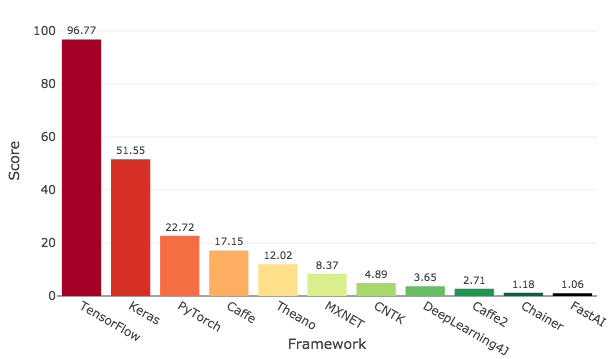
\includegraphics[width=\linewidth]{figures/dl_framework.png}
    \caption{Power score of the most deep learning frameworks in 2018}
    \label{fig:dl-frameworks}
\end{figure}

While TensorFlow is popular in the industry, another framework named Pytorch
gets more attention from academic users like the researchers. In ReID
community, most of the code is based on Pytorch, there is even no baseline
model implemented in TensorFlow and Keras for ReID task.
In contrast, since YOLO is widely used in industry, there are already tons
of existing implementations of YOLO in TensorFlow. In order to keep our
implementation consistent in one framework and reduce the overhead for
translating data from one to another, we choose TensorFlow as our deep
learning platform. By employing it, our research actually fills the gap that no
existing solution for ReID task based on TensorFlow.


\subsection{Keras}

Keras \cite{keras-framework} is a high-level open-source library written in
Python, firstly developed by Francois Chollet, which can take TensorFlow,
Theano and some other frameworks as its back-end. It doesn't provide the
mathematics operation implementation as they were left to the backend but a
human-friendly APIs which can allow you to prototype your conceptual
neural network (or other machine learning architecture) easily and experiment
with different deep learning frameworks. TensorFlow adopted Keras into its core
and announce it as the official high-level APIs in 2017 and more support are
added to Keras since TensorFlow 2.0 which was released in the middle of 2019.

\section{Summary}

In this chapter, we gave intensively review to the most common deep
learning-based methods in both object detection and person re-identification
domains.
%
For object detection problem, we started from the seminal work R-CNN
and stated the key contributions of each existing approach and compare them
with similar methods if comparable. Due to our real-time limitation from the
requirement, we are restricted to use one-stage method. Precisely, we select
YOLO v3 as our detector, because its inference time is large margin better than
all the others and the community already has a lot of existing resources of it.
%
For person re-identification problem, we introduced a total of five different models
and explain their network architectures and loss functions. Jointly considering
the trade-off between implementation complexity and the model's performance, we
decide to use the combination of the identification model and triplet model.
%
In the last part of this section, we end up with listing all the available
software we are going to employ as dependencies in our solution.

% EOF
